\begin{frame}%{\bf Schematic picture of handling input data}
\vskip-12pt
  \hskip-1cm
  \begin{tikzpicture}[node distance = 0pt, outer sep = 0pt]
    tikzstyle{every node}=[font=\tiny]
    \onslide<1->
    {
      \node[input] (inputEV) at (7.2,0.4) {Input event file};
      \node[commentDetailed, left = of inputEV, align=center] (inputEVCom) {stores tracks:\\ 4-momentum vector \\ vertex coordinates \\ particle type};
    }\onslide<2->
    {
      \node[className] (smearer) at (7.2,-1.) {TrackSmearer};
      \node[left = of smearer, xshift=-15pt] (sLEFT) {};
      \draw[arr] (inputEV) --  (smearer);
    }\onslide<2>
    {
      \node[comment, right = of smearer] (smearerCom) {called for each track};
    }\onslide<3->
    {
      \node[class, below = of smearer] (ssmear) {::Smear(Track\&)};
    }\onslide<3-7>
    {
      \node[comment, right = of ssmear] (ssmearCom) {Smears track variables\\ $\widetilde{\tau_i}=\tau_i+\rho_i$};
    }
    \onslide<4->
    {
      \node[input] (input) at (-0.5,0) {Input data file};
      \node[commentDetailed, below = of input, align=center] (inputCom) {$\eta_{min}, N_\eta, $\\$C_{0,d_0}$, ...,  \\$C_{0,\rho(d_0,\phi_0)}$,...};
    }\onslide<5->
    {
      \node[className] (manager) at (2,0) {MuonMatrixManager};
      \draw[arr] (input) --  (manager);
      \node[class, below = of manager] (minit) {::initialise()};
      \node[left = of minit, xshift=-15pt] (mLEFT) {};
    }\onslide<5-6>
    {
      \node[comment, right = of minit] (minitCom) {reads file, saves into \\MuonBinData objects};
    }\onslide<6->
    {
      \node[className] (bin) at (2,-4.3) {MuonBinData};
      \draw[arr] (minit.west) -| (mLEFT.east) |- (bin.west);
    }\onslide<6>
    {     \node[comment, right = of bin] (binCom) {stores coefficients for $\eta$ and $r_T$ bins};
    }
    \onslide<7->
    {
      \node[class, below = of minit] (mget) {::getVariables(TrackTrajectory\& track, \\CLHEP::HepSymMatrix\& sigma)};
      \draw[arr] (ssmear.west) -| (sLEFT.south) |-  (mget.east);
    }\onslide<7>
    {
      \node[comment, right = of mget] (mgetCom) {returns vector $\mathbf{\rho}$\\of 5 parameters};
    }
    \onslide<8->
    {
      \node[class, below = of mget] (mgetBinData) {::getBinData(Track\&)};
      \node[left = of mgetBinData, xshift=-5pt] (m2LEFT) {};
      \draw[arr] (mget.west) -| (m2LEFT.east) |- (mgetBinData.west);
    }\onslide<8>
    {
      \node[comment, right = of mgetBinData] (mgetBinDataCom) {returns MuonBinData \\for track's $\eta$ and $r_T$};
    }\onslide<9->
    {
      \node[class, below = of bin] (bgetMatrix) {::getMatrix(Track\&)};
      \node[left = of mget, xshift=-10pt] (m3LEFT) {};
      \draw[arr] (mget.west) -| (m3LEFT.east) |- (bgetMatrix.west);
    }\onslide<9-17>
    {
      \node[comment, right = of bgetMatrix] (bgetMatrixCom) {returns covariance matrix $\mathbf{S}$};
    }\onslide<10->
    {
      \node[className] (params) at (2.,-7) {ParameterResolution};
      \node[class, below = of params] (pres) {::resolution(Track\&)};
      \node[left = of pres, xshift=-5pt] (pLEFT) {};
    }\onslide<10-14,18->
    {
      \draw[arr] (bgetMatrix.west) -| (pLEFT.east) |- (pres.west);
    }\onslide<15-17>
    {
      \draw[->,black!20] (bgetMatrix.west) -| (pLEFT.east) |- (pres.west);
    }\onslide<10>
    {
      \node[comment, right = of pres] (presCom) {calculates $\sigma_{i}$ and $\rho_{ij}$\\ from coefficients $C_k$ \\ ($i,j=d_0,z_0,...$, $k=0,...,4$)};
    }\onslide<12-14>
    {
      \node[commentDetailed, right=of presCom, yshift=10pt] (presComCom) {slope = $\frac{C_{k,\eta_{high}}-C_{k,\eta_{low}}}{\eta_{high}-\eta_{low}}$};
    } \onslide<13-14>
    {
      \node[commentDetailed, below=of presComCom] (presComCom2) { $C_k = C_{k,\eta_{low}}+ slope\times(\eta-\eta_{low})$};
    }\onslide<14-17>
    {
      \node[commentDetailed, below=of presComCom2] (presComCom2) { $\sigma_i$ or $\rho_{ij}$ $= C_0 + C_1 p_T^{-1/2} +C_2 p_T^{-1} +C_3 p_T^{-3/2} +C_4 p_T^{-2}$};
    }\onslide<11-14>
    {
      \node[commentDetailed, above=of presComCom] (presPlot) {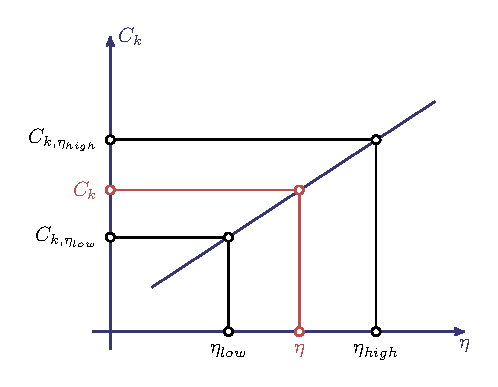
\includegraphics[width=0.25\textwidth]{plot}};
    }\onslide<11-13>
    {
      \node[comment, right = of pres] (presCom2) {linear interpolation \\for $\eta$ dependence};
    }\onslide<14>
    {
      \node[comment, right = of pres] (presCom2) {functional \\ $p_{T}$ dependence};
    }\onslide<15>
    {
      \node[commentDetailed, below = of bgetMatrix, align=center] (diagonalsMatrix) {
        $\left[\begin{matrix}
            \sigma_{d_0}^2 & . & . & . & . \\
            . & \sigma_{z_0}^2 & . & . & . \\
            . & . &  \sigma_{\phi_0}^2 &  . & . \\
            . & . & . & \sigma_{ctg\theta}^2 & . \\
            . & . & . & . & \sigma_{q/p_T}^2 \\
          \end{matrix}\right]$
      };
    } \onslide<16>
    {
      \node[commentDetailed, below = of bgetMatrix, align=center] (offdiagonalsMatrix) {
        $\left[\begin{matrix}
            . & . & \rho_{13}{\sigma_{1}\sigma_{3}} & . & \rho_{15}{\sigma_{1}\sigma_{5}}  \\
            . & . & . & \rho_{24}{\sigma_{2}\sigma_{4}}  & . \\
            . & . &  . &  . & \rho_{35}{\sigma_{3}\sigma_{5}}  \\
            . & . & . & . & . \\
            . & . & . & . & . \\
          \end{matrix}\right]$ \\
        additional checks:\\
        if square root $\mathbf{R}$ ($\mathbf{RR}=\mathbf{S}$) exists\\
        and if $\rho_{ij}\in[-1,1]$
      };

    }\onslide<17>
    {
      \node[commentDetailed, below = of bgetMatrix, align=center] (allMatrix) {
        $\left[\begin{matrix}
            \sigma_{1}^2 & . & \rho_{13}{\sigma_{1}\sigma_{3}} & . & \rho_{15}{\sigma_{1}\sigma_{5}}  \\
            . & \sigma_{2}^2 & . &  & \rho_{24}{\sigma_{2}\sigma_{4}}  & . \\
            \rho_{13}{\sigma_{1}\sigma_{3}} & . &  \sigma_{3}^2 &  . & \rho_{35}{\sigma_{3}\sigma_{5}}  \\
            . & \rho_{24}{\sigma_{2}\sigma_{4}} & . & \sigma_{4}^2 & . \\
            \rho_{15}{\sigma_{1}\sigma_{5}} & . & \rho_{35}{\sigma_{3}\sigma_{5}} & . & \sigma_{5}^2 \\
          \end{matrix}\right]$ 
      };

    } \onslide<18->
    {
      \node[className] (corr) at (6.,-2) {CorrelatedData};
      \node[class, below = of corr] (cgen) {::generate(CLHEP::HepMatrix\&)};
      \node[left = of mget, yshift=-20pt, xshift=-7.5pt] (mDOWN) {};
      \draw[arr] (mget.west) -| (mDOWN.east) |- (cgen.west);

    } \onslide<19-22>
    {
      \node[comment, right = of cgen] (cgenCom) {returns the result of $\mathbf{R} \times \mathbf{N}$};
    } \onslide<20->
    {

      \node[class, below = of cgen ] (croot) {::root(CLHEP::HepMatrix\&)};
      \node[left = of croot, xshift=-10pt] (c2LEFT) {};
      \draw[arr] (cgen.west)  -| (c2LEFT.east) |- (croot.west);
    } \onslide<20>
    {

      \node[comment, right = of croot] (crootCom) {calculates matrix $\mathbf{R}$, a square root of matrix $\mathbf{S}$ ($\mathbf{R}\mathbf{R}=\mathbf{S}$),  implementation of Cholesky decomposition};
    }\onslide<21>
    {
      \node[commentDetailed, below = of croot, align=center] (rootMatrix) {
        \scalebox{0.6}
        {
         $ \mathbf{S} =  \left[\begin{matrix}

            \sigma_{1} &  & &  &  \\

            0 & \sigma_{2} &  &   & &  \\

            \rho_{13}{\sigma_{3}} & 0 &  \sigma_{3}\sqrt{1-\rho_{13}\frac{\sigma_{1}}{\sigma_{3}}} &   & \\

            0 & \rho_{24}\sigma_{4} & 0 & \sigma_{4}\sqrt{1-\rho_{24}\frac{\sigma_{2}}{\sigma_{4}}} &  \\

            \rho_{15}\sigma_{5} & 0 & \frac{\sigma_5(\rho_{35}-\rho_{13}\rho_{15})} { 1 - \rho_{13}\frac{\sigma_{1}}{\sigma_{3}}} & . & \sigma_{5}\sqrt{1-\rho_{15}\frac{\sigma_1}{\sigma_5}-\rho_{35}\frac{\sigma_3}{\sigma_5}} \\

          \end{matrix}\right]  \left[\begin{matrix}

            \sigma_{1} & 0 & \rho_{13}\sigma_{3} & 0 & \rho_{15}\sigma_{5}  \\

             & \sigma_{2} & 0 &   & \rho_{24}\sigma_{4}  & 0 \\

            &  &  \sigma_{3}\sqrt{1-\rho_{13}\frac{\sigma_{1}}{\sigma_{3}}} &  0 & \frac{\sigma_5(\rho_{35}-\rho_{13}\rho_{15})} { 1 - \rho_{13}\frac{\sigma_{1}}{\sigma_{3}}} \\

            &  &  & \sigma_{4}\sqrt{1-\rho_{24}\frac{\sigma_{2}}{\sigma_{4}}} & 0 \\

            &  &  & & \sigma_{5}\sqrt{1-\rho_{15}\frac{\sigma_1}{\sigma_5}-\rho_{35}\frac{\sigma_3}{\sigma_5}} \\

          \end{matrix}\right]$
        }
      };

    } \onslide<22->
    {
      \node[class, below = of croot] (cnorm) {::normal(int)};
      \node[left = of cnorm, xshift=-5pt] (cLEFT) {};
      \draw[arr] (cgen.west) -| (cLEFT.east) |- (cnorm.west);
    } \onslide<22-23>
    {
      \node[comment, right = of cnorm] (cnormCom) {generates vector $\mathbf{N}$ (of 5 numbers from normal distribution)};
    } \onslide<23->
    { \node[class, below = of cnorm] (cdev) {:::makeDeviate\\(pair$<$double,double$>$,\\ double\&)};
      \draw[arr] (cdev.west)  -| (cLEFT.east) |- (cdev.west);
    } \onslide<23>
    {
      \node[comment, right = of cdev] (cdevCom) {impelementation of Fast Normal Random Number Generator \\(ALG 712 J.L.Leva)};
    }
    \onslide<24>{}


% \draw[->,redish, thick] (pres.west)  edge [bend left] node[rotate=90, yshift=5pt] {$\sigma_{i}$, $\rho_{ij}$, }  (bgetMatrix.west);
  \end{tikzpicture}
\end{frame}